\begin{doublespacing}

\section{Introduction}
Many methods are available to measure the elastic constants of solids. The resonance method was limited to specific shape and crystallographic symmetry. Using the calculus of variations the integral equations for free vibrating elastic bodies are developed. Lets assume  an arbitrarily shaped object
with elastic tensor $C_{ijkl}$ and density $\rho$ with a free surface $S$ surrounding a volume $V$. Both quantities($\rho$ and $C_{ijkl}$) may vary with the position in $V$. Let $\omega$ be a non-negative real number, \textbf{u(r)} be a real-valued function of position \textbf{r} in $V$. Then the combination of $\{\omega,\textbf{u}\}$ is a free oscillation or resonance if the real-valued displacement field satisfies
\nomenclature{$C_{ijkl}$}{stiffness tensor}
\nomenclature{\textbf{u}}{displacement vector}
\nomenclature{\textbf{s}}{surface vector}
\nomenclature{$\omega$}{angular frequency}
\nomenclature{$V$}{volume}
\nomenclature{$\mathcal{S}$}{free surface}



\begin{equation}
\textbf{s}(\textbf{r},t) = \Re(\textbf{u}(\textbf{r})e^{i\omega t})
\end{equation}
\nomenclature{$\Re$}{real number}


the elastic equations of motion in volume $V$. The analytical solution of this mechanical behavior is next to impossible \cite{zadler2004resonant}. In fact for a given volume, for all values of $\omega$ there will be no displacement (\textbf{u}) value that will satisfy the boundary condition. To solve the problem a numerical approach is used. 
%---------------------------******--------------------------
\section{Formulation of the Problem}
We consider conservative systems in which the kinetic and potential energy is function of position only. And the kinetic and potential energy is a function of resonance.
 Using classical mechanics the Lagrangian of the system is 
\begin{equation}
\label{eq_lagrangian}
\mathcal{L}=\int_V (E_k - E_p)dV
\end{equation}
\nomenclature{$\mathcal{L}$}{Lagrangian}
\nomenclature{$E_k$}{kinetic energy}
\nomenclature{$E_p$}{potential energy}


Here $E_k$ and $E_p$ are the kinetic and potential energy respectively. The potential energy associated with the displacement \textbf{u} is given by the strain energy
\begin{equation}
E_p = \frac{1}{2} \int_V C_{ijkl} \frac{\partial{u_i}}{\partial{x_j}} \frac{\partial{u_k}}{\partial{x_l}}
\end{equation}
Where $u_i$ is the \textit{i}th ($i=1,2,3 $ corresponding to the x, y or z directions in coordinate space) component of the displacement vector \textbf{u} and we have assumed that the displacements' time dependence is $e^{iwt}$. The corresponding kinetic energy will be 
\begin{equation}
E_k = \omega^2 K
\end{equation}
where
\begin{equation}
\label{eq_kmatrix}
K = \frac{1}{2} \int_V \rho u_i u_i dV
\end{equation}
Now the Lagrangian becomes (using Eq. \ref{eq_lagrangian})
\begin{equation}
\label{eq_lagrangian_2}
\mathcal{L} = \omega^2 K - E_p
\end{equation}
The kinetic and potential energy in the above equation can be calculated for any $\omega$ and $\textbf{u}$. Now it is necessary to find a condition where we can use the above equation for resonance only. In this situation classical mechanics helps by assuming that the quantity $\mathcal{L}$ is \textit{stationary} if and only if $\omega$ and $\textbf{u}$ are a resonance of V. The term \textit{stationary} implies that $\mathcal{L}$ does not change within the volume V and surface S if the displacement $\textbf{u}$ is replaced by $\textbf{u}+\partial{\textbf{u}}$.
\begin{equation}
\mathcal{L} \rightarrow \mathcal{L} + \partial{\mathcal{L}}
\end{equation}
\begin{equation}
\mathcal{L} + \partial{\mathcal{L}} = \frac{1}{2}\int_V\left[\rho \omega^2 (u_i + \partial{u_i})^2 - C_{ijkl}\frac{\partial(u_i + \partial{u_i})}{\partial{x_j}} \frac{\partial{u_k}}{\partial{x_l}} \right] dV
\end{equation}
Keeping terms to first order in $\partial{u_i}$, the change in lagrangian is 
\begin{equation}
\partial{\mathcal{L}} = \int_V \left [\rho \omega^2 u_i \partial{u_i} - C_{ijkl} \frac{\partial(\partial{u_i})}{\partial{x_j}} \frac{\partial{u_k}}{\partial{x_l}} \right ]dV
\end{equation}
After integration by parts it yields,
\begin{equation}
\label{eq_twoterms}
\partial{\mathcal{L}} = \int_V \left(\rho \omega^2 u_i + C_{ijkl} \frac {\partial^2{u_k}}{\partial{x_j}\partial{x_l}} \right )_i \partial{u_i} dV + \int_S \left (\vec{\eta}_j C_{ijkl}\frac{\partial{u_k}}{\partial{x_l}} \right)_i \partial{u_i} dS
\end{equation}
Here, $\vec{\eta_j}$ is the normal vector to the surface. The above equation (\ref{eq_twoterms}) can be written in the following form:
\begin{equation}
\partial{\mathcal{L}} = \int_V (elastic\ wave\ equation)_i \partial{u_i} dV + \int_S (surface\  traction)_i \partial{u_i} dS
\end{equation}
Due to the stationary condition the change of Lagrangian has to be zero(i.e, $\partial{\mathcal{L}}=0$). To satisfy the condition each of the two terms inside the Equation \ref{eq_twoterms} have to be independently zero. Setting the first term of the equation to zero yields the wave equation:
\begin{equation}
\label{eq_wave}
\rho \omega^2 u_i + \sum_{j,k,l}C_{ijkl} \frac{\partial^2{u_k}}{\partial{x_j}\partial{x_l}} = 0
\end{equation}
The second bracketed term is the expression of the free-surface boundary condition.
\begin{equation}
\label{eq_surface}
\sum_{j,k,l}\eta_j C_{ijkl}\frac{\partial{u_k}}{\partial{x_l}} = \sum_j\vec{\eta} \sigma_{ij}= 0
\end{equation}
\nomenclature{$\eta$}{unit vector normal to surface}
\nomenclature{$\sigma_{ij}$}{stress component}


The above equation represents the \textit{i}th component of the surface traction vector. Where $\eta_i$ is the unit vector normal to surface and $\sigma_{ij}$ is the \textit{ij} component of the stress tensor. So the displacement vector $u_i$ which satisfies these conditions (Equation \ref{eq_wave}, \ref{eq_surface}) will represent a singular value of $\omega$; which is one of the normal mode frequencies of free vibration of the system.

\subsection{Choice of Basis Function}
The next step is to turn the displacement vector \textbf{u} into some mathematical function. One way is to use a simple expansion that can satisfy a range of geometry. Using Rayleigh-Ritz method \cite{preumont2013twelve}, the displacement vector can be expanded in the following way:
\begin{equation}
\label{eq_rritz}
u_i = \sum_{\lambda} a_{i\lambda} \Phi_\lambda
\end{equation}
\nomenclature{$a_{i\lambda}$}{generalized constant}
\nomenclature{$\Phi_\lambda$}{shape function}
\nomenclature{$\lambda$}{basis set, Lam\'e constant}


Where $a_{i\lambda}$ are the generalized constants and $\Phi_\lambda$ are a set of \textit{shape functions}. Both of these are linearly independent and satisfying the global kinematic boundary condition. The choice of $\Phi_\lambda$ is arbitrary. Historically, Demarest and Ohno used normalized Legendre polynomials \cite{demarest1971cube} \cite{ohno1976free}. This had the advantage of dealing with simpler matrices, but it also limits the choice of object shape. Visscher used the following method to expand the \textit{shape function} $\Phi_\lambda$ \cite{visscher1991normal}.
\begin{equation}
\label{eq_shapefunction}
\Phi_\lambda =  x^{l(\lambda)}y^{m(\lambda)}z^{n(\lambda)}
\end{equation}
Where $(l,m,n)$ are discrete element of basis set $\lambda$ and $l, m, n \in \mathbb{Z}^+$. Equation (\ref{eq_rritz}) can be written in the following form:
\nomenclature{$\mathbb{Z}^+$}{positive integer}



\begin{equation}
\label{eq_infinity}
u_i = \sum_{(l,m,n)}^\infty a_{i(l,m,n)} \Phi_{(l,m,n)}
\end{equation}
The above equation cannot be summed to infinity, thus a truncation condition will be imposed. The truncation condition is:
\begin{equation}
\label{eq_truncation}
l+m+n \le N
\end{equation}
The truncation condition will introduce truncation error since Equation \ref{eq_infinity} is not being summed to infinity. In practice N has a number that will compromise between computational time and accuracy. It is a combination problem to find out how many polynomials will appear in the expansion of the displacement. The correct number of combinations is 
\begin{equation}
\binom{N+3}{3} = \frac{(N+3)!}{3!(N+3)!} = \frac{(N+1)(N+2)(N+3)}{6}
\end{equation}

\subsection{Lagrangian in Matrix Form}
For a given number of N  there are basis elements counting all three components of \textbf{u}. Now replacing the displacement vector (Equation \ref{eq_rritz}) with the basis function in Equation \ref{eq_lagrangian} yields the following form.
\begin{equation}
\label{eq_biglagrangian}
\mathcal{L} = \frac{1}{2} \int_V \left[\rho \omega^2 a_{i\lambda} a_{i'\lambda'} \Phi_\lambda \Phi_{\lambda'} \delta_{ii'} - \frac{1}{2} C_{ijkl} a_{i\lambda} a_{i'\lambda'} \frac{\partial{\Phi_\lambda}}{\partial{x_j}} \frac{\partial{\Phi_\lambda'}}{\partial{x_l}} \right] dV
\end{equation}
Here $\delta_{ii'}$ is a \textit{Kronecker delta}, which provides following condition
\begin{equation}
\delta_{ii'} = 
\begin{cases}
1 & \text{if i=i'} \\
0 & \text{if i$\ne$ i'}
\end{cases}
\end{equation}
\nomenclature{$\delta_{ii'}$}{Kronecker delta}


$\lambda$ and $\lambda'$ represent two different basis sets. To keep track of  all the subscripts in Equation \ref{eq_biglagrangian} the following conditions are required.
\begin{table}[H]
\centering
\begin{tabular}{l}
 $i$ the Cartesian component of \textbf{u}  \\
 $l(\lambda)$ the component of $x$ in $\Phi_\lambda$ \\
 $m(\lambda)$ the component of $y$ in $\Phi_\lambda$ \\
 $n(\lambda)$ the component of $z$ in $\Phi_\lambda$ \\
\end{tabular}
\end{table}
\noindent Equation \ref{eq_biglagrangian} can be written in the following matrix equation.
\begin{equation}
\label{eq_lagrangian_matrix}
\mathcal{L}=\frac{1}{2}\omega^2 \textbf{a}^T E \textbf{a} - \frac{1}{2} \textbf{a}^T \Gamma \textbf{a}
\end{equation}
Where \textbf{a} is a vector with elements $a_i$ whose transpose is $a^T$and where $E$ and $\Gamma$ are matrices whose order R (number of columns and rows) is determined by the truncation condition in Equation \ref{eq_truncation}. The matrix $E$ has elements
\begin{equation}
\label{eq_ematrix}
E_{\lambda i \lambda' i'} = \delta_{ii'} \int_V \Phi_\lambda \rho  \Phi_{\lambda'} dV
\end{equation}
And the matrix $\Gamma$ has elements
\nomenclature{$\Gamma$}{stiffness matrix}


\begin{equation}
\label{eq_gammamatrix}
\Gamma_{\lambda i \lambda' i'} = C_{ijkl} \int_V \frac{\partial{\Phi_{\lambda}}}{\partial{x_j}} \frac{\partial{\Phi_{\lambda'}}}{\partial{x_{j'}}} dV
\end{equation}
If $\Phi_\lambda$ was chosen to be an orthonormal set with respect to the density $\rho$ (Demarest and Ohno did using Legendre polynomials), $E$ would have been a unit matrix and our calculation would be simple. Since our choice of $\Phi_\lambda$  provides a wide range of shapes, it has computational complexity. To simplify the matrices, the following calculation can be followed. Using the $K$ matrix from Equation
\ref{eq_kmatrix}:

\begin{equation}
\begin{array}{cl}
 K &= \frac{1}{2} \int_V \rho u_i u_i dV \\
 K _{\lambda \lambda'} &= \frac{1}{2} \int_V \rho \alpha_\lambda x^{l(\lambda)} y^{m(\lambda)} z^{(\lambda)} \delta_{i(\lambda)i'(\lambda)} \times \alpha_{\lambda'} x^{l(\lambda')} y^{m(\lambda')} z^{n(\lambda')} dV \\
  &= \frac{1}{2} \int_V \rho x^{l(\lambda + \lambda')} y^{m(\lambda + \lambda')} z^{n(\lambda + \lambda')} dV 
\end{array}
\end{equation}
There is a similar but complicated expansion of matrix $E$. In both cases the result has similar integral form as follows.
\begin{equation}
\int_V f(x,y,z) x^l y^m z^n dV
\end{equation}
Where $f(x,y,z)$ is either density for matrix $E$ or one of the Cartesian components of the elastic stiffness tensor. In any region (constant S and volume V) in which $f(x,y,z)$ can be written as a monomial basis function, a condition that includes the nearly universal case of being constant in S, all of the integrals are in the following form:
\begin{equation}
\label{eq_integral}
\mathcal{I}(l,m,n) = \int_S x^l y^m z^n dV 
\end{equation}
All of these problems reduce to the evaluation of the integral from the above equation, which is sometimes referred as \textit{geometric} integral. Matrix $E$ and $\Gamma$ can be re-written in the following way.
\begin{equation}
E_{\lambda i \lambda' i'} = \int_V \rho x^l y^m z^n dV = \rho \mathcal{I}
\end{equation}
\begin{equation}
\Gamma_{\lambda i \lambda' i'}=\int_V C_{ijkl} f(x,y,z)x^l y^m z^n dV = C_{ijkl}f(x,y,z)\mathcal{I}
\end{equation}


\subsection{Generalized Eigenvalue Equation}
Equation \ref{eq_lagrangian} for Lagrangian is stationary if the displacements $u_i$ are solutions of the free-vibration problem. These solutions may be obtained by setting the derivatives of Equation \ref{eq_lagrangian_matrix} to zero with respect to each of the R amplitude  $a_{i \lambda}$. Since $\delta \mathcal{L}=0,\quad \partial \mathcal{L}/ \partial{a_{i\lambda}} = 0$, this yields the following equation: 
\begin{equation}
\label{eq_eigen}
\omega^2 E \textbf{a} =  \Gamma \textbf{a}
\end{equation}
Equation \ref{eq_eigen} is the \textit{generalized symmetric eigenvalue problem} and is readily solved with modern software. This is the ultimate equation that is solved to get the resonance frequencies. Here eigenvalues are $\omega^2$ and the eigenvectors are $\textbf{a}$. Thus, calculating the resonant frequencies for a 3D elastic body is essentially one of calculating the matrices $\Gamma$ and $E$. The special vectors \textbf{a} are the \textit{mode shapes} of the system. These are the special initial displacements that will cause the mass to vibrate harmonically.

Now the problem is reduced to correctly determining the matrices $E$ and $\Gamma$. To explain how to generate these matrices a simple geometry with high symmetry will be used. The most frequently used sample geometry for RUS is the rectangular parallelepiped (RP). Here we are assuming that the crystallographic axes align with the sample faces and with orthorhombic or higher crystal symmetry. The mathematical development is summarized in the following flow chart Figure \ref{fig_rus_flow}.\\[1.5cm]
\begin{figure}[H]
\centering
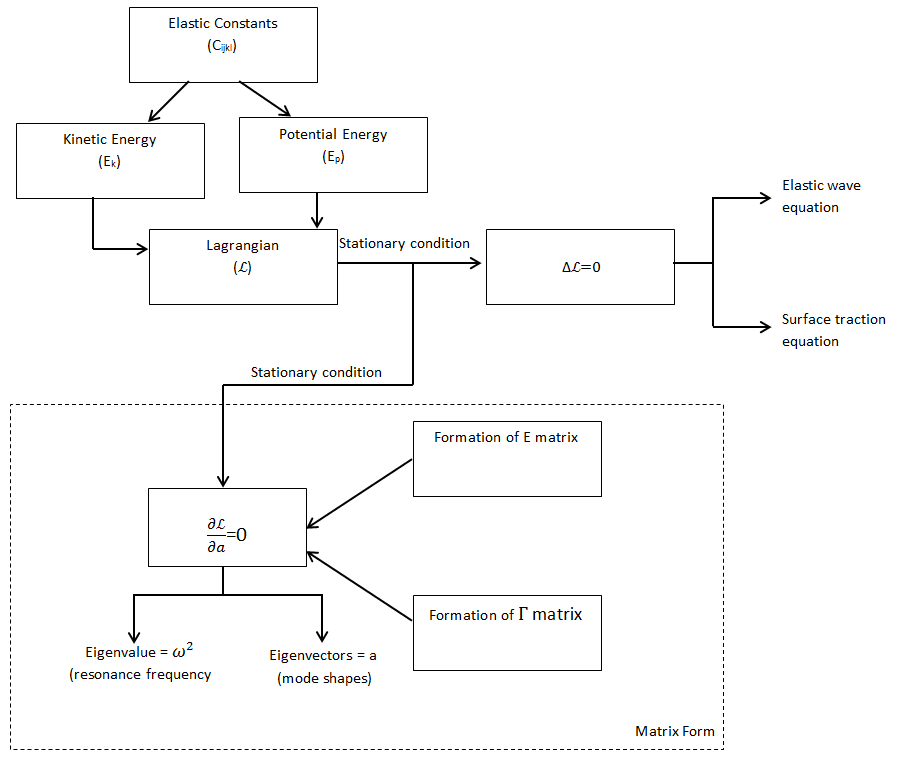
\includegraphics[scale=0.7]{rus_flow_01}
\caption{Flow chart of the mathematical development of a typical RUS problem}
\label{fig_rus_flow}
\end{figure}






\subsection{Example:Calculation of Resonance frequencies of Rectangular parallelepiped}
\begin{figure}[H]
\centering
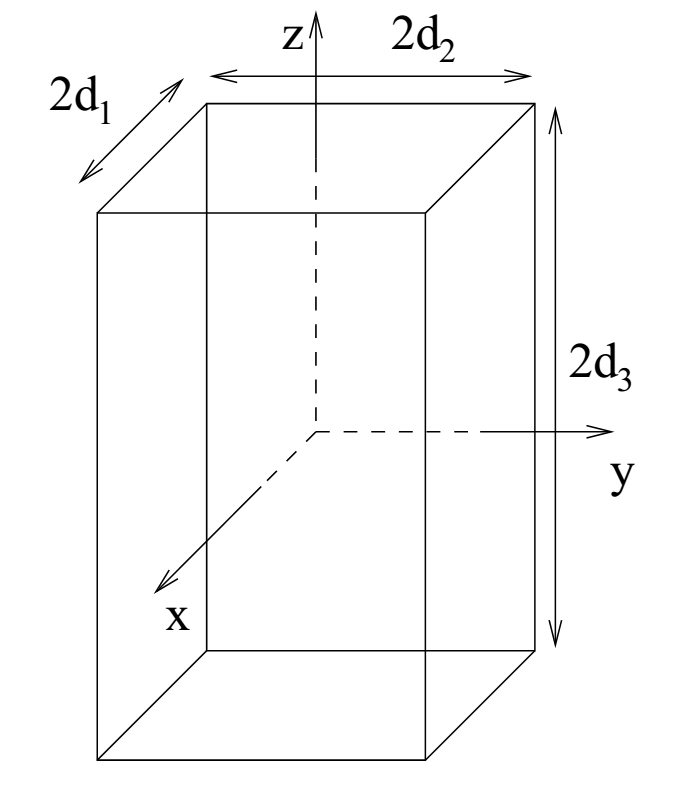
\includegraphics[scale=0.35]{RP.png}
\caption{Dimension associated with rectangular parallelepiped(RP)}
\label{fig_RP}
\end{figure}
For a RP of sides $2d_1$, $2d_2$, $2d_3$ (Figure \ref{fig_RP}), the integral in Equation \ref{eq_integral} can be evaluated explicitly to give
\begin{equation}
\label{eq_rpintegral}
\mathcal{I}(l,m,n) = \frac{8d_1^{l+1}d_2^{m+1}d_3^{n+1}}{(l+1)(m+1)(n+1)}
\end{equation}
\nomenclature{$d_1,d_2,d_3$}{sides of a rectangular parallelepiped}

To get the above integral form some assumptions were made. In order to simplify matrix $\Gamma$, we have to understand the elastic constant $C_{ijkl}$ and how it can be minimized using isotropic assumptions. To generate matrix $E$ and $\Gamma$ for rectangular parallelepiped, a Matlab code is given in appendix A. This code is written based on Visscher's XYZ algorithm \cite{visscher1991normal}. And the generalized eigen function equation solved using Matlab's \textit{eig} function.

\section{Basics of Elasticity}
When a force, either internal or external, is applied to a continuum every point of this continuum is influenced by this force. Internal force is referred as \textit{body force} and external force as \textit{contact force}. Gravity is an example of body force. Body forces are proportional to the volume of the medium and to its density. Contact forces depend on the surface they are acting on. 

If an external force acts on a continuum, it will lead to deformation (changes of size and shape) of the medium. Internal forces acting within the medium will try to resist this deformation. As a consequence the  medium will return to its original shape and volume when the external forces are removed. If this recovery of this original shape is perfect, the medium is called is \textit{elastic}. The law relating the applied force to the deformation is called \textit{Hooke's Law}. It is defined by stress and strain. Hooke's law states that the strain is linearly proportional to stress or conversely, that the stress is linearly proportional to stress \cite{auld1973acoustic}. The second form is stated by writing each component of stress (elastic restoring force) as a general linear function of all the strain components. The generalized form will be 
\begin{multline}
\sigma_{xx}=C_{xxxx}\epsilon_{xx} + C_{xxxy}\epsilon_{xy} +  C_{xxxz}\epsilon_{xz}+\\ C_{xxyx}\epsilon_{yx}+ C_{xxyy}\epsilon_{yy}+C_{xxyz}\epsilon_{yz}+\\ C_{xxzx}\epsilon_{zx}+C_{xxzy}\epsilon_{zy}+C_{xxzz}\epsilon_{zz}
\end{multline}
The above equation can be written in the following form
\begin{equation}
\label{eq_hooke}
\sigma_{ij}=C_{ijkl}\epsilon_{kl} \quad with \  i,j,k,l = x,y,z
\end{equation}
Here $C_{ijkl}$ are the components of the fourth-order \textit{stiffness} tensor of material properties or \textit{Elastic moduli}. The fourth-order stiffness tensor has 81 constants and 16 components for three-dimensional problem. The stress tensor $\sigma_{ij}$ completely describes the state of stress at any point p of the continuum.
\begin{figure}[H]
\centering
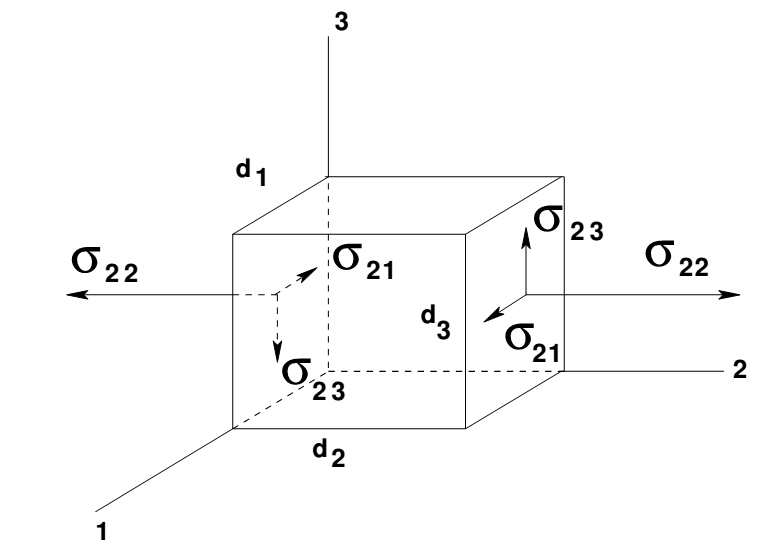
\includegraphics[scale=0.5]{stress_component.png}
\caption{Stress component on a particular point}
\label{fig:my_label}
\end{figure}
\begin{equation}
\sigma_{ij} = \left ( \begin{array}{ccc}
 \sigma_{11}& \sigma_{12} & \sigma_{13}  \\
 \sigma_{21}& \sigma_{22} & \sigma_{23} \\
 \sigma_{31}& \sigma_{32} & \sigma_{33}
\end{array}\right ) \quad with \ i,j = 1,2,3
\end{equation}
Equation \ref{eq_hooke} contains nine equations (corresponding to all possible combinations of the subscripts $ij$) and each equation contains nine strain variables. Due to the symmetry of strain and stress tensors the stiffness tensor reduces to a smaller number. Using the symmetry of stress tensor:
\begin{equation}
\sigma_{ij}=\sigma_{ji} \Longrightarrow C_{ijkl}=C_{jikl}
\end{equation}
This reduces the number of stiffness constants from $81=3\times3\times3\times3 \rightarrow 54 = 6\times3\times3$.
Similarly using the symmetry of strain tensor:
\begin{equation}
\epsilon_{ij} = \epsilon_{ji} \Longrightarrow C_{ijkl}=C_{jikl}
\end{equation}
This reduces the material constants to $36=6 \times 6$. To reduce the size of the material constants we can use the symmetry property of the tensor itself. Which is
\begin{equation}
C_{ijkl} = C_{klij}
\end{equation}
This further reduces the number of material constants to 21. The most general anisotropic (triclinic crystal structure) linear elastic material therefore has 21 elastic constants. Now the stress-strain relationship can be written as follows
\begin{equation}
\left [ \begin{array}{c}
\sigma_{11} \\ \sigma_{22} \\ \sigma_{33} \\ \sigma_{23} \\ \sigma_{13} \\ \sigma_{12}
\end{array} \right ] = \left[ \begin{array}{cccccc}
 C_{1111} & C_{1122} &  C_{1133} & C_{1123} & C_{1113} & C_{1112}\\
          & C_{2222} & C_{2233} & C_{2223} & C_{2213} & C_{2212} \\
          &          & C_{3333} & C_{3323} & C_{3313} & C_{3312} \\
          & symm     &           & C_{2323} & C_{2313} & C_{2312} \\
          &          &            &         & C_{1313}  & C_{1312} \\
          &          &           &          &           &C_{1212}
  
\end{array}  \right ] \left[\begin{array}{c}
 \epsilon_{11}\\ \epsilon_{22} \\ \epsilon_{33} \\ 2\epsilon_{23} \\ 2\epsilon_{13} \\ 2\epsilon_{12}
\end{array}    \right ]
\end{equation}
Since the $3\times3\times3\times3$ tensors become $6\times6$, we can use general matrix notation to explain the stress-strain relation. 
With these constraints on the stiffness constants the four subscript on the tensor may be reduced to two by using abbreviated subscript notation, where
\begin{table}[H]
\centering
\begin{tabular}{cc}
$I$ & $ij$  \\
$1$ & $xx$ \\
$2$ & $yy$ \\
$3$ & $zz$ \\
$4$ & $yz, zy$ \\
$5$ & $xz, zx$ \\
$6$ & $xy,yx$
\end{tabular}
\end{table}

\begin{equation}
\label{eq_stiffnessmatrix}
[C] = \left[\begin{array}{cccccc}
 C_{11} & C_{12} &  C_{13} & C_{14} & C_{15} & C_{16}\\
          & C_{22} & C_{23} & C_{24} & C_{25} & C_{26} \\
          &          & C_{33} & C_{34} & C_{35} & C_{36} \\
          & symm     &           & C_{44} & C_{45} & C_{46} \\
          &          &            &         & C_{55}  & C_{56} \\
          &          &           &          &           &C_{66}
  
\end{array}  \right]
\end{equation}
The above equation shows the elastic constants for a complete anisotropic material, which has 21 elastic constants. When the material has symmetry within its structure the number of elastic constants reduces even further.

\subsection{Elastic Isotropy Conditions}
It is necessary to determine the restrictions imposed by elastic isotropy on stiffness matrices. In an isotropic medium the three coordinates axes, x,y,z and the three coordinate planes yz, xz, xy are equivalent. This means the elastic constants are independent of the direction of the axes. Consequently, the response of the medium must be the same for a compressive stress applied along any axis. Therefore:
\begin{table}[H]
\centering
\begin{tabular}{l}
 $\epsilon_{11}=\epsilon_{22}=\epsilon_{33}$  \\
 $\epsilon_{12}=\epsilon_{13}=\epsilon_{23}$
\end{tabular}
\end{table}
 Also, the shear strain produced in a coordinate plane by a shear stress applied in that plane must be the same for all coordinate planes,
 $$
\epsilon_{44}= \epsilon_{55} = \epsilon_{66}
$$
\nomenclature{$\epsilon_{ij}$}{strain tensor}

\begin{figure}[H]
\centering
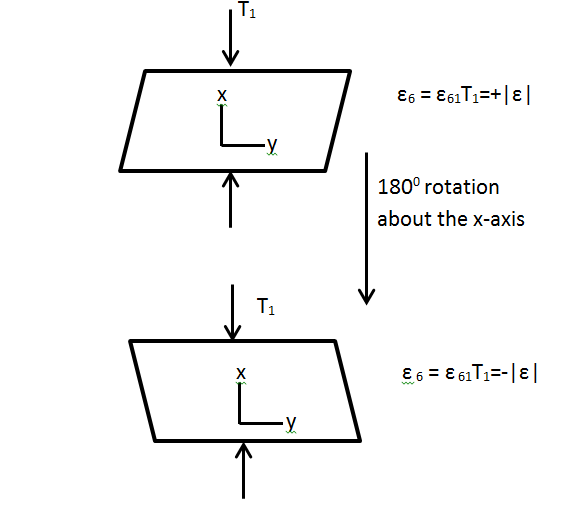
\includegraphics[scale=0.5]{sym_argument}
\caption{Symmetry logic proves that $\epsilon_{61}=-\epsilon_{61}=0$ in an isotropic medium}
\label{fig_symmetry}
\end{figure}

Now, dealing with other shear strains, suppose that a compressive stress $T_1$ applied along the $x$ axis produces a shear strain $\epsilon_6$ in the $xy$ plane. Due to the isotropic property if the plane is rotated $180^0$ about the $x$ axis, an equal valid solution to the applied stress $T_1$ will exist. This reverses the sign of the $\epsilon_6$, which can therefore only be zero. Hence
$$
\epsilon_{16}=0
$$
Similarly
$$
\epsilon_{14}=\epsilon_{15}=\epsilon_{24}=\epsilon_{25}=\epsilon_{26}=\epsilon_{34}=\epsilon_{35}=\epsilon_{36}=0
$$
Similarly using the same argument in a different coordinate plane it can be shown that
$$
\epsilon_{45}=\epsilon_{46}=\epsilon_{56}=0
$$
The above conditions can be applied to the elastic stiffness matrix (equation \ref{eq_stiffnessmatrix}). When these conditions are used the matrix becomes
\begin{equation}
\label{eq_isotropicmatrix}
[C] = \left[\begin{array}{cccccc}
 C_{11} & C_{12} &  C_{12} & 0 & 0 & 0\\
          & C_{11} & C_{12} & 0 & 0 & 0 \\
          &          & C_{11} & 0 & 0 & 0 \\
          & symm     &           & C_{44} & 0 & 0 \\
          &          &            &         & C_{44}  & 0 \\
          &          &           &          &           &C_{44}
  
\end{array}  \right]
\end{equation}
The above expression for the elastic constants may be sufficient for the isotropic material. And it is also similar to the stiffness matrix of the cubic material. But using the rotation over the $z$ axis it can be shown that\cite{auld1973acoustic} the condition for invariance of matrix [C] for an isotropic material is
\begin{equation}
\label{eq_c11c44}
C_{12}=C_{11}-2C_{44}
\end{equation}
This same condition can be obtained using rotation about the $y$ axis or $x$ axis. From equation \ref{eq_isotropicmatrix} and \ref{eq_c11c44} it is clear that for an isotropic medium there are only two independent elastic constants. These are often called \textit{Lam\'e} \textit{constants} $\lambda$ and $\mu$, defined by
\begin{table}[H]
\centering
\begin{tabular}{cc}
 $\lambda$ & $= C_{12}$  \\
 $\mu$ & $=C_{44}$
\end{tabular}
\end{table}
\nomenclature{$\mu$}{Lam\'e constant}

Using the Lam\'e constants the stiffness matrix can be represented in the following way:
\begin{equation}
[C] = \left[\begin{array}{cccccc}
 \lambda+2\mu & \lambda &  \lambda & 0 & 0 & 0\\ & \lambda+2\mu & \mu & 0 & 0 & 0 \\
          &          & \lambda+2\mu & 0 & 0 & 0 \\ &  symm     &           & \mu & 0 & 0 \\
          &          &            &         & \mu  & 0 \\  &          &           &          &          &  \mu \end{array}  \right]
\end{equation}

Lam\'e constant $\mu$ is referred to as \textit{shear modulus}, which is the measure of the shear stress. The second Lam\'e constant $\lambda$ is important as a combination with other elastic constants, e.g., the Young's modulus $E$, the bulk modulus $K$, and Poisson's ratio $\nu$. 

\subsection{Engineering Constants}
Equation \ref{eq_hooke} provides the linear relationship between stress ($\sigma_{ij}$) and strain ($\epsilon_{kl}$). Alternatively, the strains may be expressed as a general linear function of the stresses,
\begin{equation}
\epsilon_{ij}=\mathcal{S}_{ijkl}\sigma_{kl}
\end{equation}
\nomenclature{$\mathcal{S}_{ijkl}$}{complience constants}


Here $\mathcal{S}_{ijkl}$ is called \textit{compliance constants}, which is the inverse of the stiffness matrix (Equation \ref{eq_stiffnessmatrix}). That is:
\begin{equation}
[\mathcal{S}]=[C]^{-1}
\end{equation}
The compliance constants for an isotropic medium can be obtained by taking inverse of the stiffness matrix of the isotropic medium (\ref{eq_isotropicmatrix}). Matrix $C$ has dimensions of $6\times6$, so the inverted matrix will also have the same dimensions. So the compliance matrix will be 
\begin{equation}
\label{eq_isotropicmatrix}
[\mathcal{S}] = \left[\begin{array}{cccccc}
 \mathcal{S}_{11} & \mathcal{S}_{12} &  \mathcal{S}_{12} & 0 & 0 & 0\\
          & \mathcal{S}_{11} & \mathcal{S}_{12} & 0 & 0 & 0 \\
          &          & \mathcal{S}_{11} & 0 & 0 & 0 \\
          & symm     &           & \mathcal{S}_{44} & 0 & 0 \\
          &          &            &         & \mathcal{S}_{44}  & 0 \\
          &          &           &          &           &\mathcal{S}_{44}
  
\end{array}  \right]
\end{equation}
with
$$
\mathcal{S}_{11}= \frac{C_{11}+C_{12}}{(C_{11}-C_{12})(C_{11}+2C_{12})}
$$
$$
\mathcal{S}_{12} = \frac{-C_{12}}{(C_{11}-C_{12})(C_{11}+2C_{12})} $$
$$
\mathcal{S}_{44} = \frac{1}{C_{44}}
$$
\begin{figure}[H]
\centering
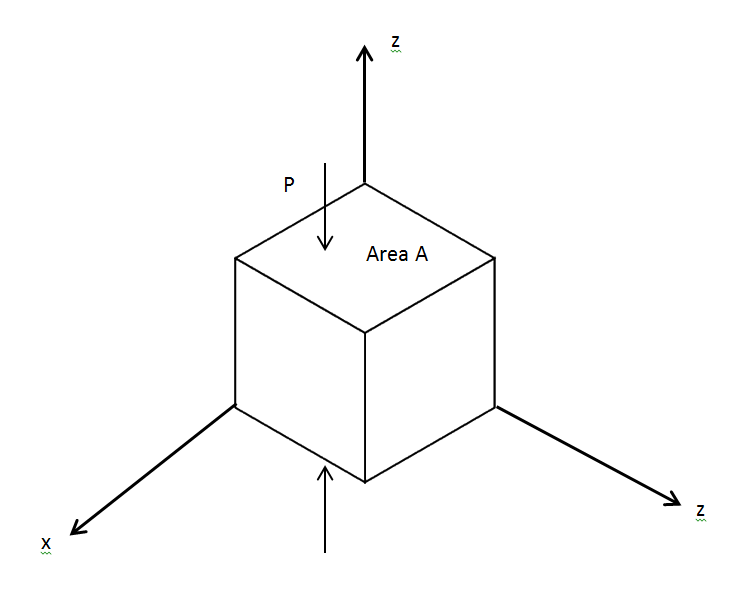
\includegraphics[scale=0.5]{fig_isotrop}
\caption{Isotropic object subjects to pressure $P$}
\label{fig_isotrop}
\end{figure}
Now, an isotropic parallelepiped (Figure \ref{fig_isotrop}) is subject to static pressure $P$ on one end and is unconstrained on its sides. Then the strain field will be: 
$$
\epsilon_{11}=\mathcal{S}_{12}\frac{p}{A}
$$
$$
\epsilon_{22}=\mathcal{S}_{12}\frac{p}{A}
$$
$$
\epsilon_{33}=\mathcal{S}_{11}\frac{p}{A}
$$
\nomenclature{$p$}{pressure}
\nomenclature{$A$}{Area}
Poisson's ratio, $\nu$, provides information about the ratio between lateral and longitudinal strain in uniaxial tensile stress. Using the condition in Figure \ref{fig_isotrop}, $\nu$ can be written in the following  form using strains:

\begin{equation}
\label{eq_poisson}
\nu =-\frac{\epsilon_{11}}{\epsilon_{33}}=-\frac{\epsilon_{22}}{\epsilon_{33}}=\frac{\mathcal{S}_{12}}{\mathcal{S}_{11}}=\frac{C_{12}}{C_{11}+C_{12}}= \frac{\lambda}{2(\lambda+\mu)}
\end{equation}
And Young's modulus is defined by
\begin{equation}
\label{eq_youngmod}
Y=\frac{\sigma_{33}}{\epsilon_{33}}=\frac{1}{\mathcal{S}_{11}}=\frac{(C_{11}-C_{12})(C_{11}+2C_{12})}{C_{11}+C_{12}}=2\mu(1+\nu)
\end{equation}

\section{Hollow Tube Geometry}
The shape of the object for RUS experiment has an important impact on the forward calculation, as it influences the mode selection. Mode shape identification and frequency analysis for different compact geometries have been done for cylinders \cite{heyliger1993elastic}, spheres \cite{lamb1881vibrations}, cubes \cite{demarest1971cube} and rectangular parallelepiped \cite{visscher1991normal}. It is also done for arbitrary shapes which is called 'potato' \cite{visscher1991normal}. The regular shapes were studied as these are the obvious choice for fundamental mechanical property studies. However, hollow cross sections were also studied in the context of carbon nano tubes, both analytically \cite{mahan2002oscillations} and numerically \cite{li2008acoustic}. Jaglinski and Wang \cite{jaglinski2011use} did a study to calculate the resonance frequencies for the hollow geometry using RUS. But they kept their experiment limited to very small object. Even though the Rayleigh-Ritz method creates mathematical complexity for the arbitrarily shaped geometry, finite element method (FEM) provides a very good solution. The fundamental assumptions of RUS is the stress free surface of the object. But a hollow geometry creates another surface inside the object. This condition makes the integration part difficult to calculate with proper boundary condition. On the other hand defining a geometry with FEM can be less arduous. Since FEM converts the system of partial differential equations to linear algebraic system, proper boundary conditions can be provided in the interested region. So for this thesis FEM was used for the calculation of the resonance frequencies. Commercial finite element package, Abaqus, is used for this purpose.

\newpage
\section{Classical Solution of Vibrating rings and tubes}
The equations of motion for an isotropic elastic medium are, 
\begin{equation}
\label{eq_navier}
(\lambda+\mu)\frac{\partial^2{u_j}}{\partial{x_j}\partial{x_i}} + \mu\frac{\partial^2{u_i}}{\partial{x_j}\partial{x_j}} = \rho \frac{\partial^2{u_i}}{\partial{t}^2}
\end{equation}
Here $\lambda$ and $\mu$ are Lam\'e constants, subscripts \textit{i} and \textit{j} are labels for spatial dimensions, ranging from 1 to 3, \textit{t} denotes time, and $\rho$ is mass density. To derive the resonant frequencies for the free vibration problem, the required boundary conditions are $\sigma_{zz} = \sigma_{zr} = \sigma_{z\theta} $ on the $z=0$ and $z=L$ surfaces, $\sigma_{rr}=\sigma_{r\theta}=0$ on the $r=a$ and $r=b$ cylindrical surfaces. There is no analytical solution for the general problem. Analytical solutions to some of the mechanical systems are presented in the following discussions.



For thin, narrow, annular rings the resonant frequencies were obtained by Hoppe in 1872 \cite{hoppe1871vibrationen}. It was done for flexural vibrations, in which flexural vibrations travel around the ring. Later, in 1889, Rayleigh \cite{rayleigh1888free} found the solution of the finite frequency spectrum regarding extensional (rod) waves. For a thin disk the in-plane vibrations are radial and torsional waves, and each of the problems can be solved separately. When these vibrations occur together the simultaneous solution of both wave equations is necessary. For short isotropic cylinders with length equal to diameter the elastic constant can be found in the following way. As torsion being the fundamental resonant mode \cite{wang2003resonant}. 
\begin{equation}
f_{torsion} = k_{sh} \sqrt{\mu/\rho}
\end{equation}
\nomenclature{$f_{torsion}$}{torsional frequency}
\nomenclature{$k_{sh}$}{shape factor}
\nomenclature{$L$}{length}
\nomenclature{$f_{flex}$}{flexural vibration frequency}
\nomenclature{$n$}{wave length on the circumference}
\nomenclature{$a$}{center line radius of the ring}
\nomenclature{$c$}{radius of the cross-section}
\nomenclature{$h$}{tube wall thickness}
\nomenclature{$f_{ext}$}{extensional vibration frequency}

Where frequency in hertz $(f=\omega/2\pi)$, $f_{torsion}$ is the resonant frequency, $k_{sh}$ is the shape factor with units of 1/m, $\mu$ is the isotropic shear modulus in pa, and $\rho$ is the material density in $kg/m^3$. For cubes \cite{demarest1971cube} $k_{sh} = \sqrt{2}/(\pi L)$ and for cylinders of length equal to diameter \cite{heyliger1993elastic}, $k_{sh}=1/(2L)$. In both cases, L is the sample length. Flexural vibrations include both displacement at right angles to the plane and twist. Flexural vibrations can be determined using following equation \cite{love2013treatise}.
\begin{equation}
f_{flex}^2 =  \frac{Ec^4}{16 \pi ma^4} \frac{n^2(n^2-1)^2}{(n^2+1)}
\end{equation}
Where the radius of the cross-section is c and the central-line radius of the ring is a. Torsional vibrations, similar to torsional vibrations of a straight rod, correspond to twist of the cross-section about its centerline. For a complete circular ring there are vibrations of this type with n wave-lengths to the circumference, and the frequency $f_{tor}$ is given by the equation \cite{love2013treatise}.
\begin{equation}
f_{tor}^2 = \frac{\mu c^2}{16\pi ma^2} (1 + \nu + n^2)
\end{equation}
Extensional vibrations are again similar to the extension of a straight rod and are given by the following equation.
\begin{equation}
f_{ext}^2 = \frac{Ec^2}{4 \pi ma^2}(1+n^2)
\end{equation}
When n=0, the tube vibrates radially so that the central-line forms a circle of periodically variable radius appearing as ring breathing, and the cross sections move without rotation. The propagation of the free harmonic waves in an infinitely long cylindrical rod has been discussed by Pochhammer \cite{pochhammer1876ueber} on the basis of the linear theory of elasticity. Gazis determined the frequency equations for several modes for long thick walled tubes under plane strain assumptions which is similar to ring bending \cite{gazis1958exact}. The analytical solutions are only presented for the shell approximation, or $ h/a \ll 1$ where $h$ is the tube wall thickness and a is the center-line radius of the ring. Extensional mode (different from previous extensional vibration) frequencies can be approximated by the following equation.
\begin{equation}
f_{ext'} = \frac{n}{2h} \sqrt{\frac{\lambda+2\mu}{\rho}}\left[1+ \frac{7-15\nu}{8(1-\nu)(n\pi)^2}\left(\frac{h}{a-h/2}\right)^2 \right]
\end{equation}
The resonant frequency for ring extensional vibration is given by the following equation.
\begin{equation}
f_{ring-ext} = \frac{1}{\pi(2a-h)} \sqrt{\frac{\mu}{\rho}}\sqrt{\frac{n^2+1}{2(1-\nu)}}
\end{equation}


\end{doublespacing}

